% !TEX root = mainthesis.tex
%Chapter 7

\renewcommand{\thechapter}{7}

\chapter{Creating topological matter with ultra-cold atoms}

Mention different kind of topological invariants. Like Chern and $Z_2$
In the remainder of the thesis I will describe two experiments 

\section{Topology in condensed matter systems}

\subsection{A brief history of topology in condensed matter}
Topological phase transitions vs. regular phase transitions?
The 2016 Nobel prize in physics was awarded to David J. Thoules, F. Duncan M. Haldane and J. Michael Kosterlitz for theoretical discoveries of topological phase transitions and topological phases of matter. Kosterlitz and Thoules first used topology to describe phase transition on 2D materials (1973, cite Long Range Order and Metastability in Two Dimensional Solids and Superfluids). A decade later Thoules, Kohomoto, Nightingale, and den Nijs explain used the topology arguments to explain the Quantum Hall effect (Quantized Hall Conductance in a Two-Dimensional Periodic Potential). In their paper they showed that the quantization of the Hall conductivity
%
\begin{equation}
	\sigma_{xy} = Ne^2/h
	\label{eq:hall_conductivity}
\end{equation}
%
is determined by the underlying topology of the band structure (how much can the Hamiltonian be deformed without closing an energy gap). N is equal to the Chern number. 

\subsection{Berry's phase and curvature, Chern numbers, etc.}
Do it like in the paper. Start with topology and geometry and move to BZ and Chern numbers. 

\subsubsection{Example: topology of a 2D electron gas}
A generic Hamiltonian for a 2D electron gas is 
%
\begin{equation}
	\hat{H}(\mathbf{k})= \mathbf{h}(\mathbf{k})\cdot\vec{\sigma}
	\label{eq:2D_Hamiltonian}
\end{equation}
%
where $\vec{\sigma}=(\sigma_x, \sigma_y, \sigma_z)$ are the Pauli matrices and $\mathbf{h}(\mathbf{k})$


Dirac points occur in band structures when there is inversion ($\mathcal{P}$) and time reversal ($\mathcal{T}$) symmetry.  $\mathcal{P}$ symmetry takes and therefore $h_z(\mathbf{k})=0$ and for small crystal momentum $\mathbf{q}$ the Hamiltonian\ref{eq:2D_Hamiltonian} resembles that of a massles Dirac fermion $\hat H(\mathbf k)=\hbar v_F\mathbf q\cdot \vec \sigma$, where $v_F$ is a velocity. The $\mathcal{T}$ symmetry can be broken for example by applying a magnetic field, in which case the degeneracy at the Dirac point is broken and \ref{eq:2D_Hamiltonian} becomes a massive Dirac Hamiltonian. 

Something about quantum spin Hall effect and spin orbit coupling?

\section{Macroscopic effects of topology}
\subsection{Edge states}
\subsection{Topological pumping}


Topological order can be found in a wide range of physical systems, from atmospheric waves~\cite{delplace_topological_2017} and photonic materials~\cite{ozawa_topological_2019} to optomechanic~\cite{peano_topological_2015}, acoustic~\cite{yang_topological_2015} and atomic systems~\cite{cooper_topological_2018}. These topological effects are quantified in terms of integer valued invariants, such as the Chern number, applicable to the quantum Hall effect~\cite{thouless_quantized_1982,haldane_model_1988}, or the $\mathbb{Z}_2$ invariant suitable for topological insulators~\cite{kane_$z_2$_2005}. Here we engineered Rashba~\cite{noauthor_realization_nodate} spin-orbit coupling for a cold atomic gas giving non-trivial topology, yet without any lattice potential. We validated our procedure by spectroscopically measuring the full dispersion relation, and located the expected single Dirac point.  We then used matter-wave interferometry to measure the geometry underlying the dispersion relation, from which we obtained the topological index.  In contrast with crystalline materials, where topological indices take on integer values, our continuum system reveals a Chern number of 1/2.



%%%%%%%%%%%%%%%%%%%%%%%%%%%%%%%%%%%%%%%%%%%%%%%%%%%%%%%%%%%%%%%%%%
%
% Introduction and context [2 paragraphs]
%
%%%%%%%%%%%%%%%%%%%%%%%%%%%%%%%%%%%%%%%%%%%%%%%%%%%%%%%%%%%%%%%%%%
The topology of Bloch bands defines integers that serve both to classify crystalline materials and to precisely specify certain properties, such as conductivity, that are independent of small changes to lattice parameters~\cite{hasan_colloquium:_2010}. Topologically non-trivial materials first found application in metrology with the definition of the von Klitzing constant as standard of resistance~\cite{klitzing_new_1980}.  Today the application of topological systems include the definition of mass standards~\cite{newell_codata_2018}, as well as spintronic devices~\cite{zutic_spintronics:_2004} and promise applications for quantum computation~\cite{nayak_non-abelian_2008}. Ultra-cold atomic systems are a proven platform for engineering topological lattices, from the Harper-Hofsdater model~\cite{miyake_realizing_2013,aidelsburger_realization_2013,noauthor_visualizing_nodate,mancini_observation_2015}, the Haldane model~\cite{jotzu_experimental_2014}, to the Rice-Mele model~\cite{lu_geometrical_2016,lohse_thouless_2016} as well as assembling spin-orbit coupled lattices without analogues in existing materials~\cite{noauthor_realization_nodate,sun_highly_2018}.

A central tenet in topological matter is the existence of integer valued `invariants' that are independent of small changes to system parameters. For an arbitrary 2-manifold $\mathcal{M}$ and a suitable choice of vector field $\mathbf{\Omega}$ the surface integral
%
\begin{equation}
	\frac{1}{2\pi}\int_{\mathcal{M}}\mathbf \Omega\cdot d\mathbf S
	\label{Eq:topology}
\end{equation}
%
serves to define both the Euler characteristic and the Chern number. When $\mathbf{\Omega}$ is equal to the local Gaussian curvature of $\mathcal{M}$, Eq.~\ref{Eq:topology} yields the Euler characteristic, an invariant related to the number of handles or genus of $\mathcal{M}$. In contrast Eq.~\ref{Eq:topology} instead gives the Chern number when $\mathcal{M}$ is a torus describing a two-dimensional Brillouin zone (BZ) and $\mathbf{\Omega}$ is the Berry curvature that characterizes the underlying quantum states. Both the Euler characteristic and the Chern number are integer valued, but the Euler characteristic depends only on the manifold $\mathcal{M}$, whilst the Chern number depends on both a vector field (the Berry curvature) and a manifold (the Brillouin zone). 

Experimental realizations of topological materials have focused on engineering different Berry curvatures in lattice systems, since $\mathcal{M}$ is always a torus. Here we show that by by eliminating the lattice potential and thereby changing  $\mathcal{M}$ from ${\mathbb T}^2$ to ${\mathbb R}^2$, i.e. from a torus to a Cartesian plane, it is possible to create topological branches of the dispersion with half-integer Chern number along with trivial branches with zero Chern number. In our experiments we created both topological and non-topological dispersions by introducing Rashba spin-orbit coupling (SOC)~\cite{campbell_realistic_2011} to a cold quantum gas.

 We engineered Rashba SOC in the continuum by resonantly coupling three internal atomic states using two-photon Raman transitions~\cite{campbell_rashba_2016} as depicted in Fig.~\ref{fig:Schematic}a,b. Going beyond earlier experiments with continuum 2D SOC~\cite{noauthor_experimental_nodate,meng_experimental_2016}, our implementation is stable against collisional decay and features reduced spontaneous emission rates. As shown in Fig.~\ref{fig:Schematic}a, the engineered system consisted of an effective spin-1/2 subspace described by a Rashba-type SOC Hamiltonian $\hat{H}_{SOC}=2\alpha/m(\q \times \ez) \cdot \hat{\boldsymbol{\sigma}}$, with added tunable higher order terms describing quadratic and cubic Dresselhaus-like SOC~\cite{campbell_realistic_2011}, along with a topologically trivial high-energy branch. Here $\alpha$ is the spin-orbit coupling strength and $\hat{\boldsymbol{\sigma}}=(\hat{\sigma}_x,\hat{\sigma}_y,\hat{\sigma}_z)$ is the vector of Pauli operators. Our engineered Rashba system had a single Dirac cone near $\q=0$, where the two lower dispersion branches become degenerate and the Berry curvature becomes singular. Each of these branches extend to infinite momentum, making the supporting manifold a plane rather than a torus.  We studied this system with two experiments: first we spectroscopically measured these dispersion branches and directly observed the predicted Dirac point and second we used quantum state tomography to reconstruct the Berry curvature and any associated Chern numbers.

%
%%%%%%%%%%%%%%%%%%%%%%%%%%%%%%%%%%%%%%%%%%%%%%%%%%%%%%%%%%%%%%%%%%
%
% Brief descrpiption of Rashba SOC: theory and implementation
%
%%%%%%%%%%%%%%%%%%%%%%%%%%%%%%%%%%%%%%%%%%%%%%%%%%%%%%%%%%%%%%%%%%

\begin{figure*}[htb]
\begin{center}
\includegraphics[width=6.in]{Figures/Chapter7/experiment.pdf}
\caption{{\bfseries a} Our engineered dispersion consisted of a two-level Rashba subspace (red and blue) with a single Dirac point for the lowest to branches and a topologically trivial higher branch (gray).{\bfseries b} We generated $xyz$ states by combining a strong bias magnetic field along $\ez$ with strong RF magnetic field along $\ex$. This states were coupled by three cross-polarized `Raman' laser beams propagating along $\ex$, $\ey-\ex$ and $-\ex-\ey$.{\bfseries c} Each pair of Raman beams was in two-photon resonance with a single transition between the $xyz$ states which we coupled with effective coupling strenghts of $(\Omega_{zx}, \Omega_{xy}, \Omega_{yz})/2\pi=\unit[(12.6(5), 8.7(8), 10(1))]{kHz}$.}
\label{fig:Schematic}
\end{center}
\end{figure*}

%%%%%%%%%%%%%%%%%%%%%%%%%%%%%%%%%%%%%%%%%%%%%%%%%%%%%%%%%%%%%%%%%%
%
% Brief details on experimental implementation
%
%%%%%%%%%%%%%%%%%%%%%%%%%%%%%%%%%%%%%%%%%%%%%%%%%%%%%%%%%%%%%%%%%%
All of our experiments started with about $1\times 10^6$ $\Rb87$ atoms in the ground state $F=1$ hyperfine manifold, just above the transition temperature for Bose-Einstein condensation.  A bias field $B_0\ez$ gave a $\omega_0/2\pi=\unit[23.9]{MHz}$ Larmor frequency along with a sizable quadratic shift of $\epsilon/2\pi=\unit[83.24]{kHz}$. An RF magnetic field oscillating at the Larmor frequency with strength $\Omega_{RF}=1.41(2)\epsilon$ \footnote{When $\Omega_{\rm RF}=\sqrt{2}\epsilon$ the $xyz$ transitions are $\omega_{ZX}=2\omega_{xy}$ and $\omega_{ZY}=3\omega_{XY}$ and our system can be described using Floquet theory.}implemented continuous dynamical decoupling (CDD)~\cite{fonseca-romero_coherence_2005}.  This generated a set of magnetic field insensitive states~\cite{trypogeorgos_synthetic_2018, anderson_continuously_2018} that we denote by $\ket{x}$, $\ket{y}$ and $\ket{z}$ as they are closely related to the $XYZ$ states of quantum chemistry~\cite{cooper_reaching_2013} rather than the conventional $m_F$ angular momentum states. We Raman-coupled atoms prepared in any of the $xyz$ states using the three cross polarized `Raman' laser beams shown in Fig.~\ref{fig:Schematic}b, tuned to the `magic zero' wavelength $\lambda_L = \unit[790]{nm}$. We tuned the Raman lasers into the tripod configuration shown in Fig.~\ref{fig:Schematic}c, bringing each pair of Raman beams into two-photon resonance with a single transition with strengths $(\Omega_{zx}, \Omega_{xy}, \Omega_{yz})/2\pi=\unit[(12.6(5), 8.7(8), 10(1))]{kHz}$ (see SM). This coupling scheme simultaneously overcomes three limitations of earlier experiments: (1) working in the same hyperfine manifold eliminates spin-relaxation collisions; (2) unlike $m_F$ states, the $xyz$ states can be tripod-coupled with lasers far detuned as compared to the excited state hyperfine splitting greatly reducing spontaneous emission~\cite{cooper_reaching_2013}; and (3) CDD renders the $xyz$ states nearly completely insensitive to magnetic field noise.

Each pair of Raman beams coupled states $\ket{i, \k}\rightarrow \ket{j, \k+\k_{i,j}}$ where $\ket{i}$ and $\ket{j}$ denote the initial and final $xyz$ states, $\k$ is the initial momentum and $\k_{i,j}=\k_i-\k_j$ is the Raman recoil momentum. The eigenstates of our Rashba SOC Hamiltonians take the form
\begin{equation}
	\ket{\Psi_n(\q)}=\sum_{j\in xyz}\sqrt{a_{n,j}(\k)}e^{i\phi_{n,j}(\k)}\ket{j,\k=\q-\k_{j}}	
	\label{Eq:Raman_wavefunction}
\end{equation}
where the quasimomentum $\q$ is a good quantum number for the laser dressed states. We see that the bare spin states $\ket{j,\k}$ therefore contribute to laser-dressed states with quasimomentum $\q=\k+\k_j$ \note{Need to clarify this}. We leveraged the wide momentum distribution of a non-condensed ensemble ($T\approx\unit[180]{nK}$ and $T/T_c\approx 1.1$) to sample a wide range of momentum states simultaneously. Furthermore, by starting separately in each of the $xyz$ states we sampled the range of initial quasimomentum states shown in Fig.~\ref{fig:fourier_spectroscopy}a, where three Gaussian distributions corresponding to initial $xyz$ states are shifted from $\q=0$ by a Raman wave vector $\k_{X,Y,Z}$. 

Our measurement protocol consisted of first abruptly removing the confining potential and the Raman lasers, initiating a $\unit[21]{ms}$ time-of-flight (TOF). During this TOF we adiabatically transformed each of the $xyz$ states back to a corresponding $\ket{m_F}$ state and applied a `Stern-Gerlach' gradient. Finally we used resonant absorption imaging to measure the resulting density distributions, yielding the spin-resolved momentum distribution.

%%%%%%%%%%%%%%%%%%%%%%%%%%%%%%%%%%%%%%%%%%%%%%%%%%%%%%%%%%%%%%%%%%
%
% Results I: Fourier spectroscopy
%
%%%%%%%%%%%%%%%%%%%%%%%%%%%%%%%%%%%%%%%%%%%%%%%%%%%%%%%%%%%%%%%%%
\begin{figure*}[htb]
\begin{center}
\includegraphics[width=6.in]{Figures/Chapter7/fig2_v4.pdf}
\caption{{\bfseries a} The initial $xyz$ states $\ket{j,\k}$ were mapped to to laser-dressed states with quasimomentum $\q=\k+\k_j$. We used non-condensed atoms with a broad momentum distribution($T\approx\unit[180]{nK}$ and $T/T_c\approx 1.1$) and performed our experiments starting separately in each of the $xyz$ states, sampling a large range of quasimomentum states.{\bfseries b} Fourier spectroscopy protocol. We applied the Raman beams for a variable time $t_{\mathrm{p}}$: a Rabi-type atomic interferometer analogous to a three-port beam splitter.{\bfseries c} Probabilities as a function of quasimomentum for a fixed Raman pulse time $t_{\rm p}=\unit[420]{\mu s}$ {\bfseries d} Dynamics of the final populations of the $xyz$ states with quasimomentum $(q_x, q_y)=\unit[(-0.18, -0.55)]{k_{\rm L}}$ after initializing the system in the $\ket{z}$ state.}
\label{fig:fourier_spectroscopy}
\end{center}
\end{figure*}
\begin{figure}[htb]
\begin{center}
\includegraphics[width=3.1in]{Figures/Chapter7/Fourier_spectroscopy_v2.pdf}
\caption{{\bfseries a} Fourier spectra as a function of $q_y$ for fixed $q_x=-0.09$, and $0.65\,k_{\rm L}$ which we obtained by Fourier transforming the populations in the $xyz$ states as a function of $t_{\mathrm{p}}$. The dashed lines correspond to the energy differences of our model.{\bfseries b} Dispersion relation obtained from three-level model the blue and orange arrows indicate energy differences that appear as peaks in the PSD.}
\label{fig:fourier_spectroscopy_bands}
\end{center}
\end{figure}
We directly measured the 2D dispersion relation using Fourier transform spectroscopy~\cite{valdes-curiel_fourier_2017}. In this technique we considered the evolution of an initial state $\ket{i,\mathbf{k}}$ suddenly subjected to the Raman coupling lasers. This atomic Rabi-type interferometer is analogous to a three-port beam-splitter depicted in Fig.~\ref{fig:fourier_spectroscopy}b. During a pulsing time $t_{\mathrm{p}}$ we followed the dynamics of the populations in the $xyz$ states which evolved with oscillatory components proportional to $\sum_{j\neq n} a_{n,j}(\k)\cos((E_n-E_{j})t_{\mathrm{p}}\,/\hbar)$, with frequency components determined by the eigenenergy differences present in the Hamiltonian. Fig.~\ref{fig:fourier_spectroscopy}c shows the momentum dependent populations for a fixed pulse time $t_{\mathrm{p}}$ and Fig.~\ref{fig:fourier_spectroscopy}d shows representative final populations as a function of $t_{\mathrm{p}}$ for a fixed quasimomentum state. We Fourier transformed the populations in all states to produce the spectrograms displayed in Fig.~\ref{fig:fourier_spectroscopy_bands}a. These 2D spectrograms are each a cut through a 3D volumetric distribution, and together show the presence of a single Dirac point in the Rashba subspace. The dashed curves depict the energy differences from the dispersion of our full three-level system shown in Fig.~\ref{fig:fourier_spectroscopy_bands}b, and are in good agreement with our experiment. This measurement directly confirms the expected set of energies, including the existence of a two-state subspace approximately described by the Rashba Hamiltonian. However, the energies shed no light on the topology of the different branches of the dispersion which instead requires knowledge of the eigenstates. 
%
%%%%%%%%%%%%%%%%%%%%%%%%%%%%%%%%%%%%%%%%%%%%%%%%%%%%%%%%%%%%%%%%%%
%
% Results II: Measurement of Chern number
%
%%%%%%%%%%%%%%%%%%%%%%%%%%%%%%%%%%%%%%%%%%%%%%%%%%%%%%%%%%%%%%%%%%
\begin{figure*}[htb]
\begin{center}
\includegraphics[width=6.in]{Figures/Chapter7/fig3_v3.pdf}
\caption{{\bfseries a} Experimental protocol for three arm Ramsey interferometer (not to scale). (Top) We started with atoms in state $\ket{z,y,\q_i=\k+\mathbf{k}_j}$ and with detuning $\delta_y=\pm \unit[5]{E_{\rm L}}$ and $\delta_z=\pm\unit[5]{E_{\rm L}}$. We ramped the Raman beams on in $750 \us$ and then ramped the detuning back nominally zero. We let the system evolve in the dark for times between $5 \,\us$ and $400\,\us$, followed by a $\unit[25]{us}$ Raman pulse. (Bottom) The implemented experimental protocol was equivalent to a three-arm interferometer that split an initial state into three final states with amplitudes related to the initial wave function phases. {\bfseries b} Probabilities as a function of quasimomentum for the three output ports of the interferometer at $t_{\rm free}=\unit[160]{\mu s}$ {\bfseries c} Probabilities as a function of free evolution time $t_{\mathrm{free}}$ for an input state with quasimomentum $(q_x, q_y)=(-0.92, 0.55)\,k_{\rm L}$ and in the Rashba ground state.}
\label{fig:Ramsey_ramps}
\end{center}
\end{figure*}
%
\begin{figure}[htb]
\begin{center}
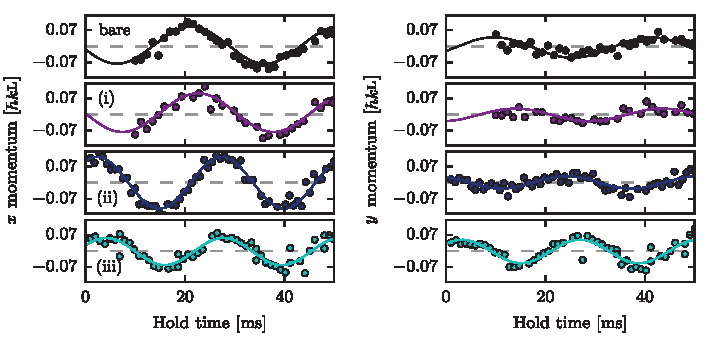
\includegraphics[width=3.3in]{Figures/Chapter7/Fig4.pdf}
\caption{{\bfseries a} Fitted phases {\bfseries b} Phase differences around a loop for three of some radius. {\bfseries c} Asymptotic Chern numher as a function of loop radius.}
\label{fig:Ramsey_phases}
\end{center}
\end{figure}
The Berry curvature present in Eq.~\ref{Eq:topology} can be derived from the Berry's connection $\mathbf{A}_n(\q)=i\bra{\Psi_n(\q)}\mathbf{\nabla}_q\ket{\Psi_n(\q)}$ which behaves much like a vector potential in classical electromagnetism. The Berry curvature $\mathbf{\Omega}_n(\q)=\mathbf{\nabla}_q\times\mathbf{A}(\q)$ is the associated magnetic field and the flux within any region is the line integral of $\mathbf{A(\q)}$ along the boundary of $\mathcal{M}$ \footnote{We assume that the line integral excludes contribution of singularities from Dirac strings.}. The Berry connection derived from Eq.~\ref{Eq:Raman_wavefunction}
%
\begin{equation}
 \mathbf A_n(\q)= -\!\!\!\!\!\!\sum_{j \in\{x, y, z\}}  a_{n,j}(\q)  \nabla_q \phi_{n,j}(\q)
\label{Eq:Berry_connection1}
\end{equation}
%
shows that knowledge of both the phase and amplitude of the wave function is required. We obtained $a_{n,j}(\q)$ and $\phi_{n,j}(\q)$ using a three arm time-domain Ramsey interferometer, implementing a variant of quantum state tomography~\cite{flaschner_experimental_2016,godfrin_generalized_2018}. Similarly to optics, the use of a multi-path interferometer allowed us to transduce initial information about complex phases into final state probabilities, which we readily obtained from absorption images. Fig.~\ref{fig:Ramsey_ramps}a shows our experimental protocol. First we combined ramps of Raman coupling strength and Raman detuning such that we adiabatically mapped an initial $\ket{j, \k}$ state into a corresponding eigenstate $\ket{n,\q=\k+\k_j}$, either in the topologically trivial highest dispersion branch ($n=3$) or in the topological ground state ($n=1$), see SM. We suddenly turned off the Raman coupling, thereby allowing the three bare state components of the Rashba eigenstates to undergo free evolution for a time $t_{\mathrm{free}}$, constituting the three arms of our time-domain interferometer. Finally we applied a three-port beam splitter using a brief Raman `recombination’ pulse to make the three arms interfere. At the end of this procedure, the population in a final state $\ket{l}$ is
\begin{equation}
P_l(\q,t)=\sum_{i\neq j} a_{n,i}a_{n,j}\cos(\omega_{i,j}(\q) t+\phi_{n,i}(\q) - \phi_{n,j}(\q)+\phi_{l,i,j}^{p}(\q))
\label{Eq:Ramsey_evolution}
\end{equation}
which directly reads out the phase differences, independent of the output port $l$. Here $\phi_{l,i,j}^{p}(\q)$ is a smoothly varying phase imprinted by the recombination pulse and is independent of $\q$ for an infinitely short and strong pulse. The angular frequencies $\omega_{i,j}(\q)=\hbar \q \cdot \k_{i,j}/m + \delta_{i,j}$ result from the known free particle kinetic energy and detuning from the tripod resonance condition. Fig.~\ref{fig:Ramsey_ramps}b shows the momentum-dependent populations in each output port at fixed $t_{\rm free}=\unit[160]{us}$ and Fig.~\ref{fig:Ramsey_ramps}c show the populations as a function of $t_{\mathrm{free}}$ for a representative quasimomentum state $(q_x, q_y)=(-0.92, 0.55)\,k_{\rm L}$. We obtained the relative phases from Eq.~\ref{Eq:Ramsey_evolution} by fitting the measured probabilities to the sum of three cosines with known frequencies but unknown amplitudes and phases. 

Fig.~\ref{fig:Ramsey_phases}a shows typical phase-maps for both the no-topological and topological branches. In the non-topological phase-maps the momentum dependence of the recombination pulse $\phi_{l,i,j}^{p}(\q)$ causes a smooth variations of the phases along the Raman recoil axes that do not affect the topological index of our system. The topological phase-maps present discontinuities along two lines in addition to the recombination pulse induced variations. We recovered the phases of the full spinor wave function from the relative phases obtained from the fits by choosing a gauge (see SM). We then used the values of $a_{n,q}$ obtained from measuring the populations in the $xyz$ states at $t_{\mathrm{free}}=0$ in combination with the phases of the wave function to compute the Berry connection~\cite{fukui_chern_2005}. Fig.~\ref{fig:Ramsey_phases}b shows the three phase differences as a function of polar angle for a loop of radius $q\approx 0.77\,k_{\rm L}$ for both the topological and non-topological branches. The phases of the topological branch have two discontinuous changes that lead to non-zero Berry phases when the Berry connection is integrated along a closed loop in momentum space. Fig.~\ref{fig:Ramsey_phases}c shows the integrated Berry phase as a function of loop radius. The largest value of $t_{\mathrm{free}}$ in the experiment limits how well we can resolve the phases of small frequency oscillations as well as different frequency components that are close to each other. This limitation is reflected in the large variation in the Berry phase shown in the shaded region of Fig.~\ref{fig:Ramsey_phases}c near $q=0$. For loops with $q>0.4\,k_{\rm L}$ we obtain an integrated Berry phase $\Phi_{\rm B}/2\pi=0.01(1)$ for the non-topological branch and $\Phi_{\rm B}/2\pi=0.51(4)$ for the topological branch. %The measured Berry phase asymptotically approaches the Chern number for increasing loop radius which and in our case its value remains the same for $q>0$

In conventional materials -- for example graphene, or the topological Haldane model -- it is well established that individual Dirac points each contribute a Berry's phase of $\Phi_{\rm B} /2\pi =\pm 1/2$, but crystalline materials conspire for these to appear in pairs, always delivering integer Chern numbers. In contrast, our system in the continuum contains a single Dirac point, resulting in a non-integer Chern number. Some work has been done in the context of electromagnetic waveguides to extend the use of Chern invariants and the bulk-edge correspondence principle to systems in the continuum~\cite{silveirinha_chern_2015}. 
%
%The Chern number can be interpreted as the magnetic flux from Dirac monopoles in momentum space through the manifold defined by the BZ. For closed manifolds such as a torus, the Chern number is always an integer. However, for an open manifold such as the plane defined by the BZ of our system in the continuum only half of the flux from the Dirac monopole is captured, resulting in a half-integer valued Chern number. 

%%%%%%%%%%%%%%%%%%%%%%%%%%%%%%%%%%%%%%%%%%%%%%%%%%%%%%%%%%%%%%%%%%
%
% Outlook
%%%%%%%%%%%%%%%%%%%%%%%%%%%%%%%%%%%%%%%%%%%%%%%%%%%%%%%%%%%%%%%%%%
Our new cold-atom implementation of Rashba SOC has the advantages of reduced losses from spin-relaxation collisions and increased stability against environmental fluctuations due to the clock-like nature of the $xyz$ sates. We measured a single Dirac point and for the first time characterized the topology of an atomic system in the continuum. The measured spontaneous emission limited lifetime of our system is $\unit[320(17)]{ms}$. However it gets reduced to $\unit[40(2)]{ms}$ when the Raman couplings are resonant which we attribute to technical noise in the relative phase between the RF field and the Raman beams, which has caused considerable consternation in ongoing experiments. A possible future direction for this work is to study interfaces between topologically inequivalent continuous media and observe emerging edge sates [ref?]. Furthermore, the ground state of our system can have three nearly degenerate minima and could allow the study of rich ground state physics in many body systems of bosons, for example the formation of fragmented BECs~\cite{stanescu_spin-orbit_2008} when the system does not condense into a single-particle state. 
%
%%%%%%%%%%%%%%%%%%%%%%%%%%%%%%%%%%%%%%%%%%%%%%%%%%%%%%%%%%%%%%%%%%


\subsection{System preparation}
Our experiments began with $N\approx 1\times 10^6$  $\Rb87$ atoms in a crossed optical dipole trap~\cite{lin_rapid_2009}, with frequencies $(f_x,f_y,f_z) \approx \unit[(70, 85, 254)]{Hz}$. We initially prepared the atoms in the $\ket{F=1, m_F=-1}$ state of the $5S_{1/2}$ electronic ground state. We then prepared atoms either in the $m_F=0$ or $m_F=+1$ state by applying an RF field with approximately $\unit[20]{kHz}$ coupling strength and ramping a bias magnetic along $\ez$ from $B_i-\unit[3.6\times 10^{-2}]{mT}$ to $B_i=\unit[3.391]{mT}$ in $\unit[50]{ms}$. We prepared the $xyz$ states by starting in each of the $m_F$ states in a bias field $B_0-\unit[7.2]{mT}$ and then ramping on the RF dressing field to $\Omega_{RF}=\unit[117.72]{kHz}$ in $\unit[1]{ms}$ and then ramped the bias field to its final value $B_0=\unit[3.4030]{mT}$ in $\unit[3]{ms}$. We finally waited for $\unit[40]{ms}$ for the fields to stabilize prior to applying any Raman coupling. 


\subsection{Raman coupling the $xyz$ states}

The energies of the $xyz$ states are $\omega_X=0$ and $\omega_{Z,Y}=-(\epsilon\pm\sqrt{4\Omega_{RF}^2+\epsilon^2})/2$. We set the frequencies of the Raman lasers to $\omega_X=\omega_L+\omega_0+\omega_{XY}$, $\omega_Y=\omega_L+\omega_0$ and $\omega_Z=\omega_L-\omega_{ZX}$,  where $\omega_L=2\pi c/\lambda_L$ and $(\omega_{ZX}, \omega_{XY}, \omega_{zy})/2\pi = \unit[(166.47, 83.24, 249.71)]{kHz}$ are the transition energies between pairs of dressed states which are integer multiples of $\epsilon$.

The Raman coupled states are well described by the kinetic and light-matter Hamiltonian 
\begin{equation}
	\hat H(\q) =\sum_{i\in\{XYZ\}}\bigg(\frac{\hbar^2(\q-\k_i)^2}{2m}+\hbar\delta_i\bigg)\ket{i}\bra{i}+\sum_{i\neq j}\hbar\Omega_{i,j}\ket{j}\bra{i},
	\label{Eq:Rashba_atoms}
\end{equation}
where $\k_i$ are the Raman wave vectors, $\delta_i$ is a detuning from Raman resonance and $\Omega_{i,j}$ is the Raman coupling strength between a pair of RF dressed states. 

\subsection{Floquet effects}
We operated in a regime where the transition energies between the $xyz$ statest were integer multuples of $\omega_{xy}$ $\omega_{zx}=2\omega_{xy}$ and $\omega_{zy}=3\omega_{xy}$, therefore we must use Floquet theory for a complete description of our system. The Hamiltonian in Eq.~\ref{Eq:Rashba_atoms} is therefore an effective Hamiltonian that describes the stroboscopic dynamics of the full Floquet Hamiltonian. We observed that the effective Raman coupling strengths for the driven three level system differed from our calibrations which were performed by only driving one pair of states because of the presence of nearby quasi-energy manifolds. This effect is mitigated for larger values of $\omega_{xy}$ as the spacing between quasi-energy manifolds is increased. 
%
\subsection{State preparation for Ramsey interferometer}

%TODO incorporate top sentence into text
For the Rashba dressed states preparation we started with RF dressed states with a different coupling strength $\Omega_{RF}\pm \unit[20]{kHz}$. This change shifted the energies of the $\ket{z}$ and $\ket{y}$states by about $\pm \unit[18.8]{kHz}$. The change in the RF dressed state eigenenergies corresponds to non-zero $\delta_Z$ and $\delta_Y$in Eq.~\ref{Eq:Rashba_atoms}. We chose the detuning such that the initial state had a large overlap with either the $n=1$ or the $n=3$ eigenstates of Eq.~\ref{Eq:Rashba_atoms}. We ramped the Raman on in $\unit[750]{\mu s}$ and then ramped $\Omega_{RF}$ to its final value in $\unit[1]{ms}$, effectively ramping $\delta_Z$ and $\delta_Y$ close to zero. This detuning ramp had the additional effect of moving the location Dirac point through the atoms, thereby creating a trajectory where the state preparation was not adiabatic. This trajectory depended on the sign of the detuning ramp and therefore we used different initial states and detuning ramps for the ground state preparation and we excluded the Dirac point trajectories when combining the data. Near the final location of the Dirac point the state preparation can not be adiabatic regardless of the initial state or detuning used for the ground state preparation.  Finally, because for our state preparation method we could not change the energy of the $\ket{x}$ we could only prepare dressed states in either the $n=1$ or $n=3$ by initializing the system in the $\ket{y}$ or $\ket{z}$ states. When we prepared the system in $\ket{x}$ the final dressed state corresponded to the $n=2$ branch.


\subsection{Obtaining phases from phase differences}
The desired phase difference are independent of the final state $\ket{l}$ and because each Raman beam addresses two different transitions between the $xyz$ states the phases are constrained such that $\sum_{i>j}\phi_{i,j}=0$.




